\section{Experimental Results}
Typical results from early materials can be found it Fig. 7. For additional data and complete testing curves, see \cite{sThesis} and \cite{mThesis}.

Since the circuitry has control over the output current and compliance voltage, it sets a limit for the maximum power allowed to be dissipated in its last pass transistor. This worst case operating method ensures that data taken of an unknown device will not damage the circuitry.
\begin{figure}[here]
\centering
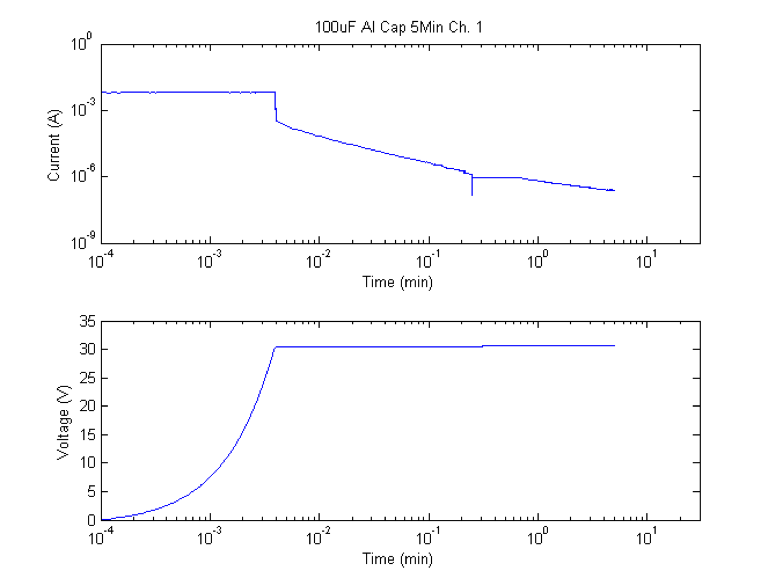
\includegraphics[width=3.5in]{measData}
\caption{Typical Results}
\label{fig:measData}
\end{figure}

